\titledquestion{Level Order Traversal}

\textbf{Level Order Traversal}

Recall the problem of \textit{tree traversal}, which is the problem of visiting
the elements of a tree in some prescribed order.

We have discussed several tree traversals, such as \textit{postorder},
\textit{inorder}, and \textit{preorder}, which are classic recursive traversals.
Less straightforward is what is known as a \textit{level-order traversal}, which
traverses a tree in the same way that a human would read a book.

\begin{center}
  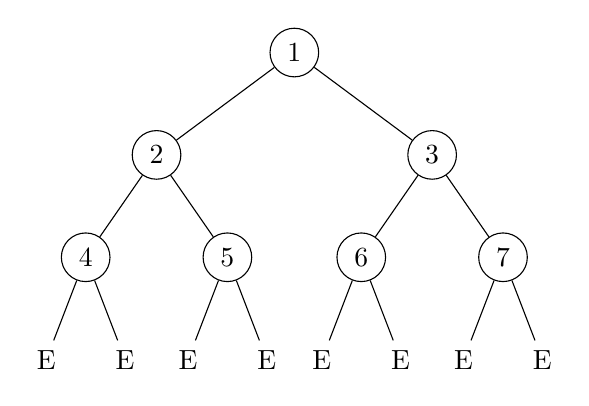
\begin{tikzpicture}[
          level 1/.style={sibling distance=35mm},
          level 2/.style={sibling distance=18mm},
          level 3/.style={sibling distance=10mm},
          level distance=13mm,
          circ/.style={draw=black, circle}
        ]
    \node[circ] {1}
      child{node[circ] {2}
        child{node[circ] {4}
          child{node {\code{E}}}
          child{node {\code{E}}}
        }
        child{node[circ] {5}
          child{node {\code{E}}}
          child{node {\code{E}}}
        }
      }
      child{node[circ] {3}
        child{node[circ] {6}
          child{node {\code{E}}}
          child{node {\code{E}}}
        }
        child{node[circ] {7}
          child{node {\code{E}}}
          child{node {\code{E}}}
        }
      }
    ;

  \end{tikzpicture}
\end{center}

This is quite difficult to implement, recursively, via naively computing
the level order traversal of children. However, by changing our perspective,
it turns out we can actually still solve this recursively.

We will do this by writing the following helper:
\spec
  {levelord}
  {\code{'a tree -> 'a list stream}}
  {\code{true}}
  {\code{levelord T} evaluates to the stream \code{S}, such that the
  $i$th element of \code{S} contains all of the elements in the $i$th
  level of the tree \code{T}.}

So for instance, if \code{T} is the above tree, we should have that:
\begin{itemize}
  \item \code{levelord T} $\eeq$ \code{Stream.fromList [[1],[2, 3],[4, 5, 6, 7],[]]}
  \item \code{levelord Empty} $\eeq$ \code{Stream.fromList [[]]}
  \item \code{levelord (N(E,1,E))} $\eeq$ \code{Stream.fromList [[1], []]}
  \item \code{levelord (N(N(E,2,E),1,E))} $\eeq$ \code{Stream.fromList [[1], [2], []]}
\end{itemize}

(The empty lists are because the corresponding level of the tree still has stuff
in it, it's just all \code{Empty}s)

\newpage

We will also give you this helper function, which you will need:

\spec
  {zipAppend}
  {{\small\code{'a list stream -> 'a list stream -> 'a list stream}}}
  {\code{true}}
  {\code{zipAppend S1 S2} evaluates to the stream which pairs up elements from
  \code{S1} and \code{S2}, appending their corresponding lists. If one doesn't
  exist in one of the streams, it simply takes the other list.}

\begin{codeblock}
  fun zipAppend S1 S2 =
    case (S.expose S1, S.expose S2) of
      (S.Empty, _) => S2
    | (_, S.Empty) => S1
    | (S.Cons (x, S1'), S.Cons (y, S2')) =>
        S.cons (x @ y, zip S1' S2')
\end{codeblock}

\begin{parts}
  \part[3]\hfill
    Is \code{zipAppend} maximally lazy? If not, explain why, and how it may be fixed.

    \begin{solutionorbox}[8em]
      No, because it exposes the streams before an element is requested.
      You should instead write:

      \begin{codeblock}
        fun zipAppend S1 S2 =
          S.delay (fn () =>
            case (S.expose S1, S.expose S2) of
              (S.Empty, _) => S2
            | (_, S.Empty) => S1
            | (S.Cons (x, S1'), S.Cons (y, S2')) =>
                S.cons (x @ y, zip S1' S2')
          )
      \end{codeblock}
    \end{solutionorbox}
  \part[12]\hfill

    Implement \code{levelord} as described above.

    \textbf{Hint:} This problem is about reasoning via specification. Do not get
    lost in the nitty gritty. Think recursively.

    This problem can be solved in three lines.

    \begin{solutionorbox}[12em]
      \begin{codeblock}
        fun levelord Empty = S.cons ([], S.empty)
          | levelord (Node (L, x, R)) =
              S.cons ([x], (zipAppend (levelord L) (levelord R)))
      \end{codeblock}
    \end{solutionorbox}

  \newpage

  \part[3]\hfill

    Assume you are given a function \code{flatten' : 'a list stream -> 'a list},
    which takes a stream of lists and flattens it into a list.

    Implement \code{levelord' : 'a tree -> 'a list}, finally, in terms of
    the functions that we have used previously.

    \begin{constraint}
      You may not use any \code{fun} declarations or \code{fn} expressions.
    \end{constraint}

    \begin{solutionorbox}[8em]
      \begin{codeblock}
        val levelord' = flatten' o levelord
      \end{codeblock}
    \end{solutionorbox}
\end{parts}

\newpage
